\chapter{Моделирование}
\section{Инструменты моделирования}
Для нахождения позиции оптимального совмещения волноводов, необходимо смоделировать поле волновода, и вычислить интеграл перекрытия, формула которого приведена в главе \ref{coupling}. Перебирая варианты взаимного расположения полей, необходимо найти максимальное значение этого интеграла.

Перебор всех теоретически возможных вариантов занимает длительное время, поэтому стоит его упростить, предполагая единственный максимум у функции. Для оптимизации поиска экстремумов функции используют методы координатного спуска, градиентного (наискорейшего) спуска и симплекс-метод. \cite{numeric} 

Предполагая, что у искомого распределения значений интеграла перекрытия имеется только один максимум, используем метод градиентного спуска, поскольку в этом случае он позволит достичь результата за меньшее число итераций. \cite{mathews}

Итак, нам нужен инструмент, позволяющий считать интегралы, проводить итерации и строить графики. В работе используется язык программирования Python, имеющий все необходимое. 

Для решения наших задач, к Python подключаются следующие внешние библиотеки:
\begin{itemize}
	\item NumPy - пакет функций для базовых операций с матрицами (создание и итерация по ним)
	\item SciPy - пакет математических функций, используется для интегрирования и содержит реализацию алгоритма градиентного спуска
	\item Matplotlib - для вывода полученных результатов в виде графиков.
\end{itemize}

Кроме того, для повышения производительности программы, были написаны два вспомогательных модуля, описывающих распределение полей канального и цилиндрического волноводов.

\section{Метод градиентного спуска}
При дальнейших расчетах имеет значение нахождение максимального значения рассматриваемых функций.
Для оптимизации поиска этих значений и сокращения перебора вариантов, был выбран метод градиентного спуска, как наиболее эффективный для функций с единственным максимумом. 

Основная его идея состоит в том, чтобы двигаться к минимуму в направлении наиболее быстрого убывания функции, которое определяется антиградиентом, то есть вектором, противоположному по направлению градиенту функции:
\begin{equation}
\mathrm{grad}\,\varphi = \nabla f = \frac {\partial f} {\partial x} \vec e_x + \frac {\partial f} {\partial y} \vec e_y + \frac {\partial f} {\partial z} \vec e_z.
\end{equation}

Нахождение минимума функции начинается с выбора каким-либо способом начальной точки, и вычисления в ней градиента рассматриваемой функции. Затем сделаем небольшой шаг в обратном, антиградиентном направлении. В результате мы придем в точку, в которой значение функции будет меньше первоначального. В новой точке повторим процедуру: снова вычислим градиент функции и сделаем шаг в обратном направлении. Продолжая этот процесс, мы будем двигаться в сторону убывания функции. Специальный выбор направления движения на каждом шаге позволяет надеяться на то, что в данном случае приближение к наименьшему значению функции будет более быстрым, чем в методе покоординатного спуска, в котором движение происходит только вдоль одной из осей координат.

Метод градиентного спуска требует вычисления градиента целевой функции на каждом шаге. Если она задана аналитически, то это, как правило, не проблема: для частных производных, определяющих градиент, можно получить явные формулы.

Достоинством метода наискорейшего спуска является его простота. Однако он имеет существенный недостаток. Это — одношаговый метод, в котором при выборе точки очередного испытания $x_{r+1}$ не используется информация о предыдущих испытаниях, кроме испытания в точке $x_r$. Для устранения этого недостатка, связанного с игнорированием информации о предыдущих испытаниях, можно использовать алгоритм, реализующий градиентный метод с памятью, в котором при выборе очередного приращения $\Delta x_r$ учитывается информация о приращении $\Delta x_{r-1}$ на предыдущем шаге. Для этого потребуем, чтобы на каждой итерации приращение $\Delta x_r$ выбиралось таким образом, чтобы обеспечивалась наибольшая скорость уменьшения функции $Q(x)$ при условии, что квадрат модуля разности приращения $\Delta x_r$ и взвешенного приращения $\Delta x_{r-1}$ оставался равным постоянной величине.

В результате выполнения этого алгоритма, мы находим точку экстремума функции и в этом случае градиентный спуск закончен, а текущие координаты точки и есть искомый результат. Следует заметить, что для поиска максимума функции можно использовать этот же алгоритм, если рассматриваемую функцию заменить на функцию с противоположным знаком.

\section{Интерактивная модель}
Для решения основной задачи, то есть поиска точки контакта с максимальным значением коэффициента передачи, было написано отдельное приложение.

\begin{figure}[h!]
	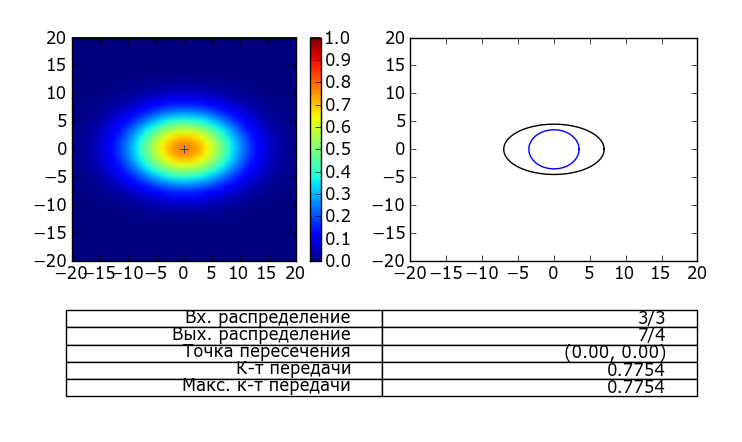
\includegraphics[width=\linewidth]{img/heatmap.pdf}
	\caption{Общий вид программы}
\end{figure}

На рисунке показан расчет эффективности стыковки, волокна ОВССП к полосковому волноводу. Цифрой 1 отмечено результирующее поле, возбужденное в планарном волноводе. Распределение показано в относительных единицах, нормированных к максимально возможному значению в этом планарном волноводе. Цифрой 2 отмечена схема перекрытия исходных полей волноводов. Внизу в таблице отмеченной цифрой 3 выводятся численные значения. Показывается радиус волокна, участвующего в расчете, координаты центра волокна, и рассчитывается коэффициент передачи. Также определяется точка стыковки с наибольшим значением интеграла перекрытия, и полученный результат отображается в последней строке. Схема интерактивная, можно выбирать точку контакта и получать результат для этого положения.

\section{Моделирование поперечного смещения}
\label{transverse_section}

Для нахождения точки максимальной эффективности передачи возьмем планарный волновод неподвижным относительно осей координат. Цилиндрический волновод будем перемещать по оси $x$. При смещении волновода максимум распределения также смещается относительно исходного на расстояние $\Delta x$, как показано на рисунке \ref{intersection}. Для исследования коэффициента передачи была написана программа, вычисляющая значения интеграла перекрытия в пределах $x \in [-20, 20]$, мкм.

В моделировании использовались волокна, описанные в \ref{cylinder_field}, которые стыковались к полосковому волноводу, описанному в \ref{strip_field}.

\begin{figure}[h!]
		\includegraphics[width=0.7\linewidth]{img/transversal_courning.png}
		\caption{Зависимость коэффициента передачи из волокна Corning}
\end{figure}
\begin{figure}[h!]
		\includegraphics[width=0.7\linewidth]{img/transversal_fog.png}
		\caption{Зависимость коэффициента передачи из волокна ОВССП}
		\label{transversal_fog}
\end{figure}
\begin{figure}[h!]
		\includegraphics[width=0.7\linewidth]{img/transversal_panda.png}
		\caption{Зависимость коэффициента передачи из волокна PANDA}
		\label{transversal_panda}
\end{figure}

В ходе моделирования, было обнаружены точки наилучшего контакта. Кроме того была обнаружена зависимость коэффициента передачи от радиуса моды. Во втором случае, показанном на рисунке \ref{transversal_fog} максимальное значение составило 79,1\%. Следовательно, возникает задача поиска наилучшего с точки зрения эффективности передачи радиуса моды. Для этого построим график зависимости максимумов передачи для радиусов моды в интервалах от 1~мкм до 7~мкм включительно.
\begin{figure}[h!]
		\includegraphics[width=0.7\linewidth]{img/var_radius.png}
		\caption{Коэффициент передачи для разных радиусов мод}
\end{figure}

В ходе моделирования получились результаты для радиусов мод несколько реальных волокон, а также найден радиус максимального контакта, в при котором происходит почти полная передача энергии - это 2,4~мкм для данного полоскового волновода. Но на таких радиусах очень велики собственные потери на данной длине волны - 1.55 мкм, поэтому идеальное значение радиуса моды, пригодное для практического применения оказывается равным примерно 4.5 мкм. Такой радиус имеет волокно ОВССП. В дальнейшем, при моделировании, мы будем использовать только его, зависимости на разных радиусах аналогичны, однако данное волокно наиболее интересно, поскольку показало наибольшую эффективность передачи на этом этапе моделирования.

\section{Моделирование продольного смещения}

При продольном смещении необходимо решить задачу нахождения вида пучка на некотором расстоянии от выхода волновода, после чего подставить получившееся распределение в интеграл перекрытия (\ref{coupling_natural}) и определить эффективность передачи.
В моделировании будем использовать канальный волновод, описанный в \ref{strip_field} и цилиндрический с радиусом моды 3~мкм и показателем преломления сердцевины $n$ = 1.47. Длину волны света примем $\lambda$ = 1.55~мкм.

\begin{figure}[h!]
	\includegraphics[width=0.7\linewidth]{img/longitudinal.png}
	\caption{Коэффициент передачи в зависимости от расстояния между волноводами}
	\label{longitudinal}
\end{figure}

По результатам моделирования получился ожидаемый результат. Эффективность передачи падает по мере увеличения расстояния между волноводами. Наибольшее значение как и в предыдущем эксперименте, составило 0.791, поскольку по осям $(x,y)$ мы взяли точку с наивысшим коэффициентом передачи.   

\section{Моделирование углового смещения}

В моделировании будем использовать титан-диффузионный оптический канальный волновод на подложке из монокристалла ниобата лития, описанный в \ref{strip_field} и оптическое волокно, спроектированное специально для ВОГ, описанное в \ref{cylinder_field}. Будем рассматривать поворот в двух плоскостях, YZ и XZ, обозначения осей показаны на рисунке \ref{polozok}б. При угловом смещении последовательно берутся разные углы стыковки, для которых моделируется поле на выходе из такого волокна и рассчитывается эффективность передачи. Поскольку мы рассматриваем цилиндрическое волокно, то углы будем брать только положительные, так как при отрицательных углах получается симметричная зависимость.

\begin{figure}[h!]
	\includegraphics[width=0.7\linewidth]{img/angular.png}
	\caption{Коэффициент передачи при разных углах стыковки без скоса}
	\label{angular}
\end{figure}

Сначала смоделируем угловое смещение для волокна без скоса. На рисунке \ref{angular} показан результат моделирования, где видно, что эффективность передачи уменьшается очень сильно и, начиная с угла в $2^\circ$, передача становится неэффективной. Теперь рассмотрим случай со скосом волокна, показнный на рисунке \ref{angular_bevel}. В этом случае эффективность остается высокой, даже на больших углах смещения.

\begin{figure}[h!]
	\includegraphics[width=0.7\linewidth]{img/angular_bevel.png}
	\caption{Коэффициент передачи при разных углах стыковки волокна со скосом}
	\label{angular_bevel}
\end{figure}

\section{Расчет отражений}
Для получения полного представления об эффективности передачи на разных углах, необходимо добавить учет обратных отражений, способ расчета которых показан в \ref{backreflection_method}. Построим график зависимости уровня обратных отражений $C_{back}$ от угла скоса. Для этого будем находить по формуле Френеля (\ref{frenel_ref}) коэффициент отражения $R$ при текущем угле скоса, и эффективность перехода в обратное распространение $C_{ref}$, а итоговое значение обратных отражений будет являться их произведением:
\begin{equation}
	C_{back} = C_{ref} \cdot R
\end{equation}

Полученная зависимость показана на рисунке \ref{backreflection}.

\begin{figure}[h!]
	\includegraphics[width=0.7\linewidth]{img/backreflection.png}
	\caption{Обратные отражения при разных углах скоса}
	\label{backreflection}
\end{figure}

По итогам моделирования выяснилось, что, поскольку коэффициент отражения на небольших углах для данных волноводов составляет около 4\%, то доля обратных отражений убывает с ростом угла скоса и после $10^{\circ}$ составляет пренебрежимо малое количество. 

Также, вследствие отражения, не весь свет пропускается дальше, а значит оказывает влияние на эффективность стыковки с полосковым волноводом. Построим график зависимости коэффициента пропускания и общей эффективности стыковки с его учетом от угла скоса.

\begin{figure}[h!]
	\includegraphics[width=0.7\linewidth]{img/angular_reflection.png}
	\caption{Эффективность передачи при разных углах скоса}
	\label{backreflection}
\end{figure}

По графику видно, что с увеличением угла стыковки возрастают отражения и пропускание оказывает все более заметное влияние на эффективность стыковки, поэтому не рекомендуется сильно увеличивать угол стыковки.